\documentclass[../main.tex]{subfiles}
\chapter{Simulation}
\label{c:simulation}

\begin{figure}
	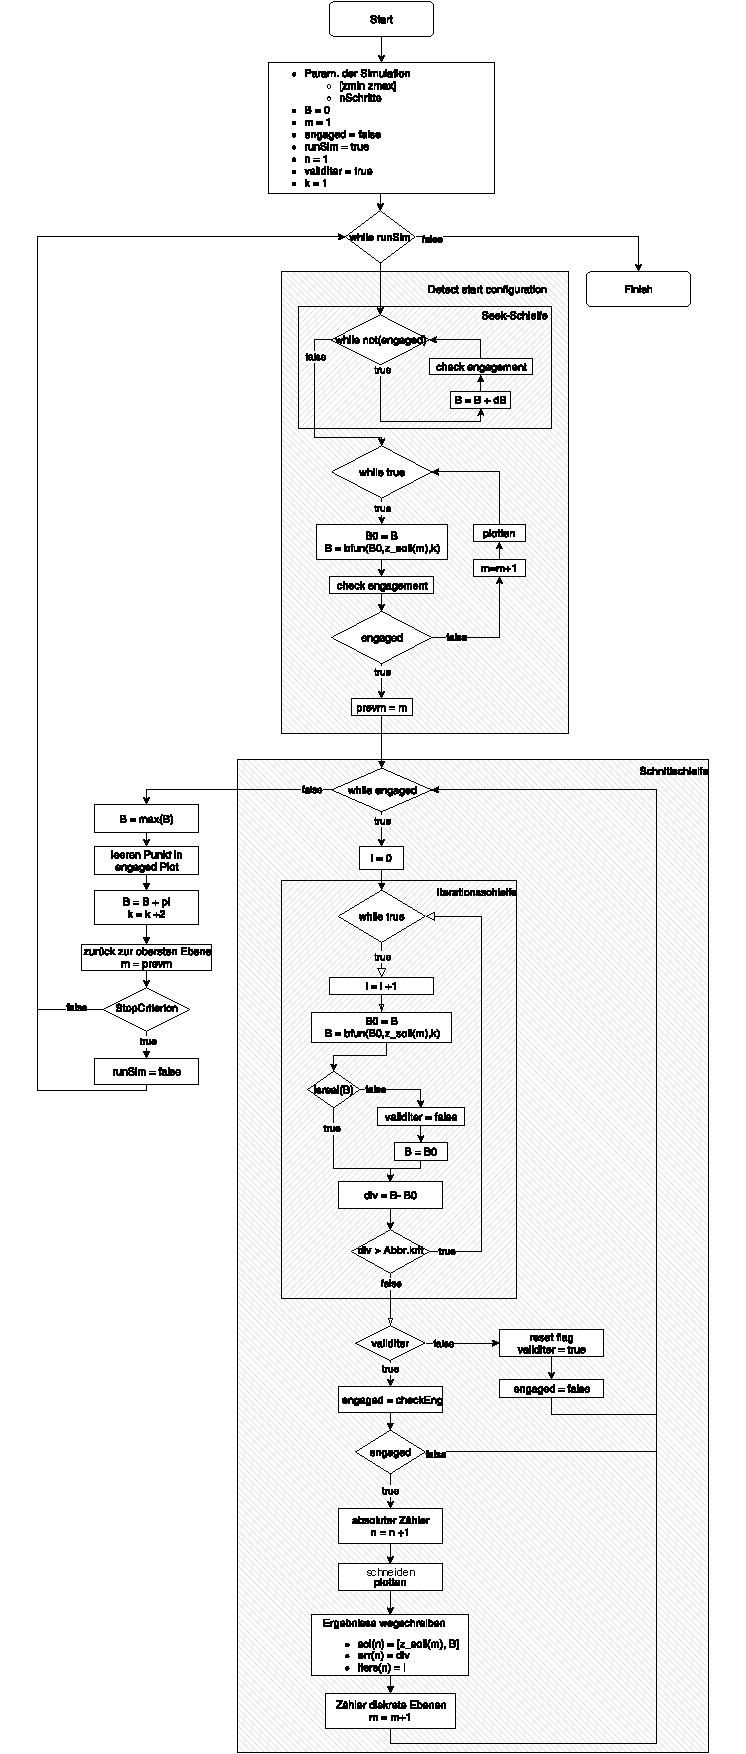
\includegraphics[scale=0.75]{vf1-flowchart}
	\caption{Hier ist die caption}
	\label{fig:flowchart}
\end{figure}

Abbildung \ref{fig:flowchart} zeigt das Flussbild der Simulation.
Der Ablauf der Simulation ist unterteilt in die Abschnitte Seeken, Findung der obersten Schnittebene, Durchführung der Schnitte mit den Lösungsiterationen, Erkennung des Schnittendes sowie Nachbereitung des Schnittes und schließlich Abschluss der Simulation.
Neben der Ausführung des Simulationscodes sollte der Status der Berechnung in Form von grafischen Ausgaben dargestellt werden.
Das Plotten von Daten in Echtzeit ist schwierig zu realisieren in \matlab, vor Allem bei dreidimensionalen Datensätzen.
Die standardmäßig zur Verfügung gestellten Routinen sind nicht gut optimiert für schnelle Ausführungszeit und es ist notorisch schwierig \matlab Code multithread-fähig zu gestalten.
Die Lösungsansätze um trotz dieser Herausforderungen die für die grafische Ausgabe beanspruchte Rechenzeit effizient zu nutzen und die Simulation möglichst geringfügig zu belasten wird ebenfalls besprochen.


Die einzelnen Prozessschritte der Simulation werden im Folgenden erläutert.

\section{Vorbereitung der Simulation}
Vor Beginn der Simulation wird die Simulationssteuerungsparameter eingelesen.
Dabei werden zunächst die Eingabedaten des betrachteten Falles festgelegt.
Mit folgende Parameter kann definiert werden, wie dieser Fall gestaltet ist:
\begin{itemize}
	\item Zähnezahl des Zahnrades
	\item Modul des Zahnrades
	\item Geometrie des des Werkzeuges (Durchmesser, Kopf- und Fußhöhe)	
\end{itemize}
Aus diesen Parametern können weitere Startbedingungen ermittelt werden.
So ist die Startposition des Werkzeugs und den daraus folgenden Positionen der Maschinenkomponenten zu berechnen wie sie in Abschnitt \ref{c:maschkomppos} besprochen wurden.
Die Position der X-Achse der Maschine wird berechnet über den Achsabstand des gedachten Schneckengetriebes nach \cite[Gleichung 23.4]{Matek2017}:
\begin{equation*}
	a = \frac{d_{s1}+d_{s2}}{2}
\end{equation*}
\begin{eqdscr}{$d_{s1}$, $d_{s2}$}
	\item[$a$] Achsabstand
	\item[$d_{s1}$, $d_{s2}$] Teilkreisdurchmesser von Schneckenrad und Schnecke
\end{eqdscr}
Der Teilkreisdurchmesser des Schneckenrades wird berechnet nach \cite{Matek2017}:
\begin{equation*}
	d_{s1} = m \cdot z
\end{equation*}
\begin{eqdscr}{$m$}
	\item[$m$] Modul
	\item[$z$] Zähnezahl des Werkstückes
\end{eqdscr}


\section{Plotten}
Die Architektur des Codes erlaubt das parallel zum Lösen des mathematischen Problems die Ausgabe erfolgt mit minimalem Einfluss auf die Ausführungsgeschwindigkeit der Berechnung.
Das wurde erreicht durch die Auslagern des Plottens in eine Klasse.
